

\begin{figure*}[t!]
    \centering
    \begin{subfigure}[b]{0.4\textwidth}
    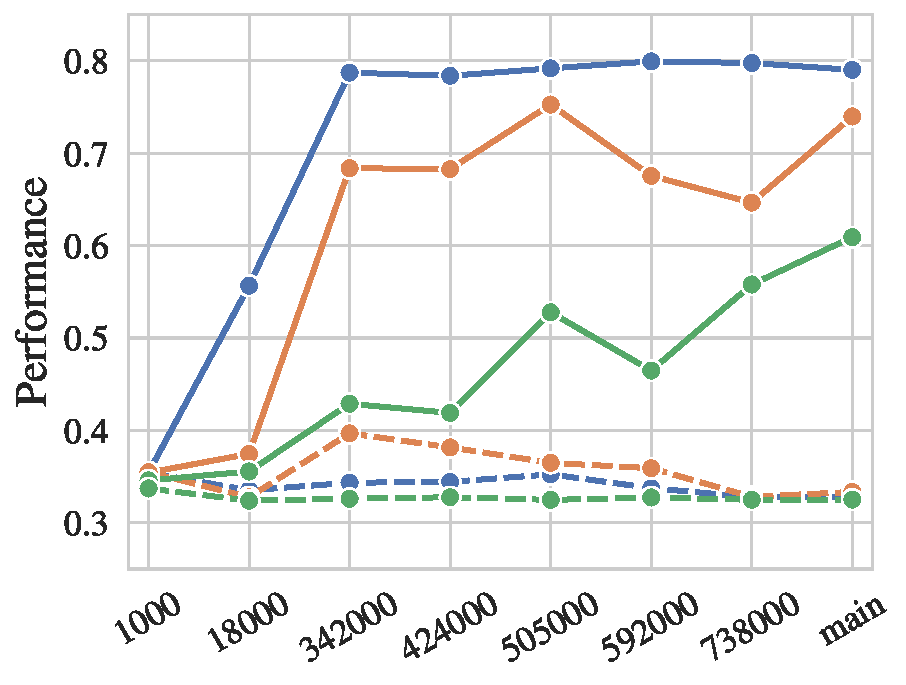
\includegraphics[width=\the\columnwidth]{figures/fig_files/task_format/task_format_evalmnli_matched-trainmnli.pdf}
        \caption{MNLI matched}
    \end{subfigure}%
    ~ 
    \begin{subfigure}[b]{0.4\textwidth}
    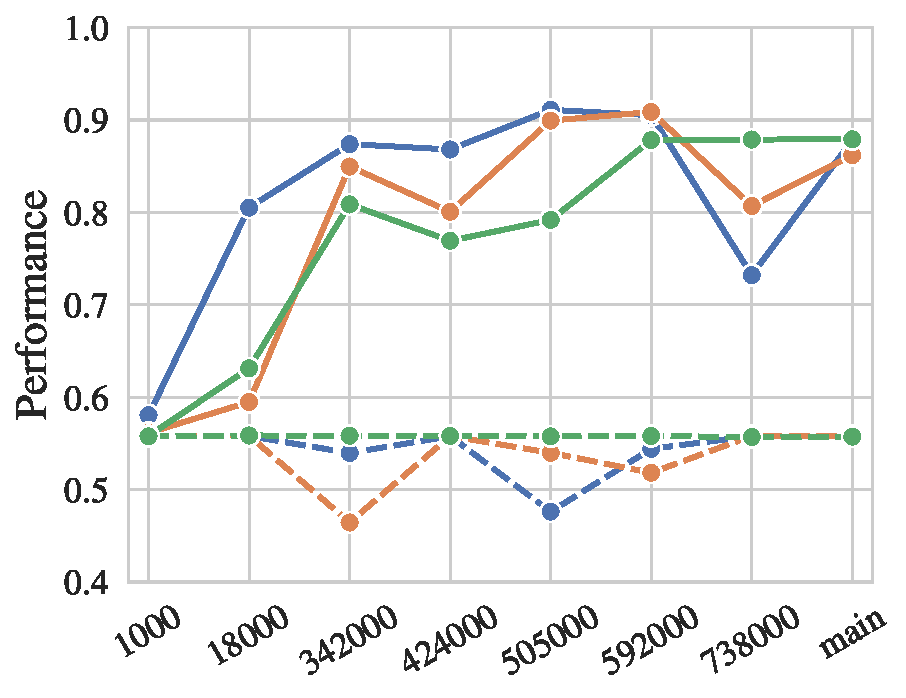
\includegraphics[width=\the\columnwidth]{figures/fig_files/task_format/task_format_evalpaws-trainpaws.pdf}
        \caption{Paws}
    \end{subfigure}%
    \\
    \begin{subfigure}[b]{0.4\textwidth}
    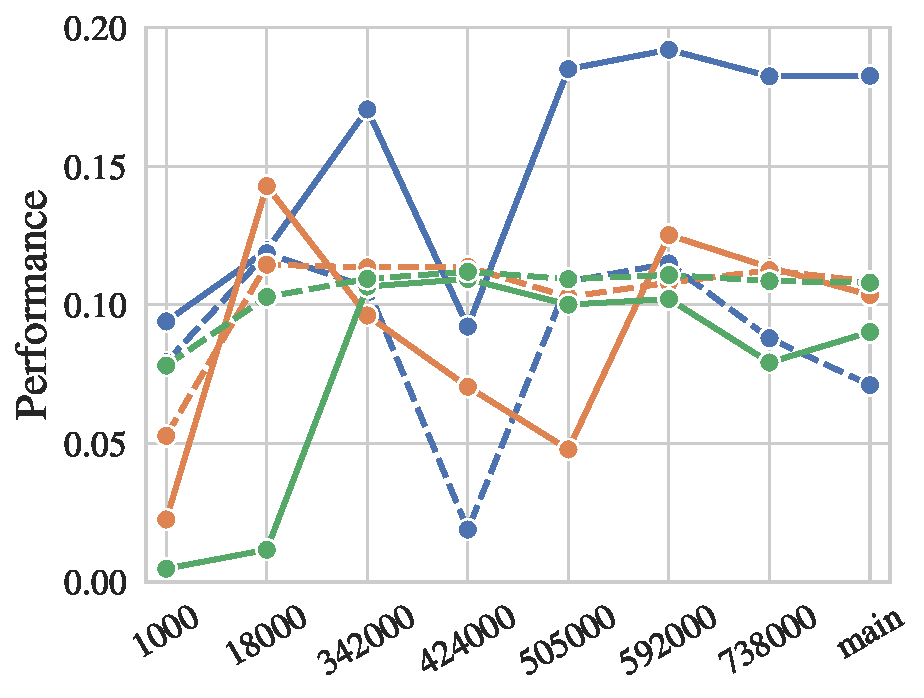
\includegraphics[width=\the\columnwidth]{figures/fig_files/task_format/task_format_evalxsum-trainxsum.pdf}
        \caption{XSum}
    \end{subfigure}%
    ~ 
    \begin{subfigure}[b]{0.55\textwidth}
    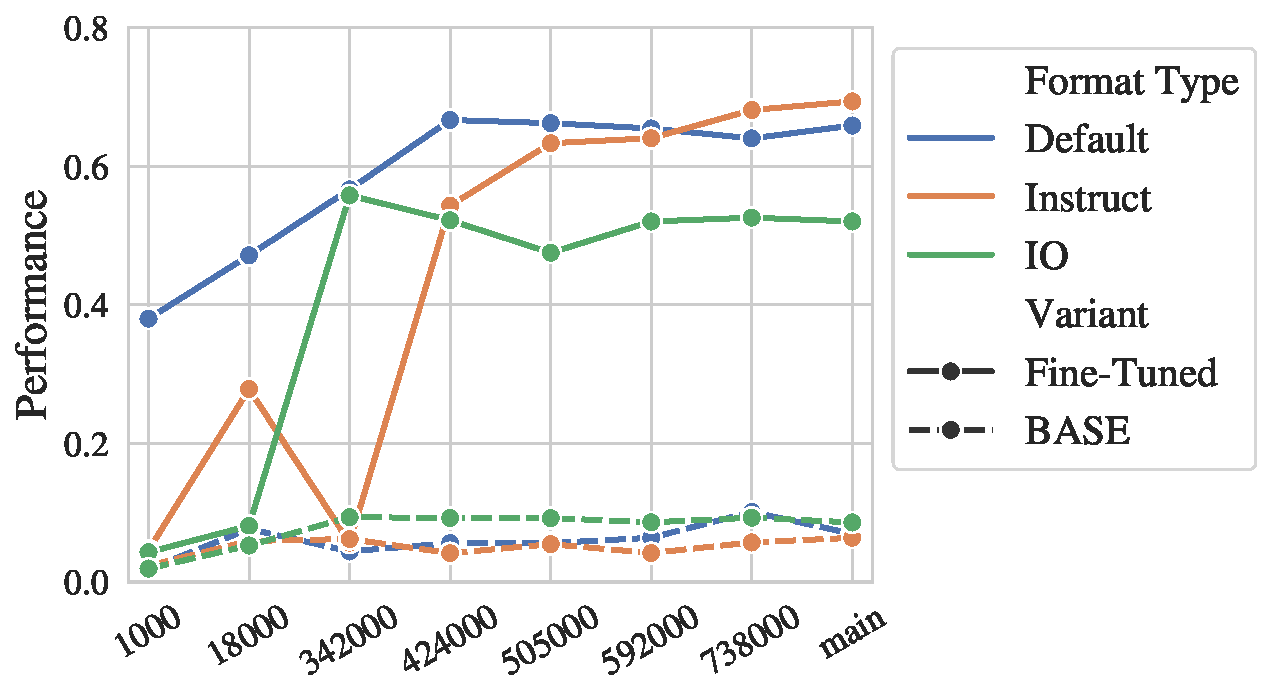
\includegraphics[width=\the\columnwidth]{figures/fig_files/task_format/task_format_evalsocialiqa-trainsocialiqa.pdf}
        \caption{SocialIQa}
    \end{subfigure}%

    \caption {Model performance with different task formats. }
  \label{fig:app:task_format}
\end{figure*}